\documentclass[aspectratio=169,11pt]{beamer}
\usetheme{Madrid}
\usecolortheme{seahorse}
\setbeamertemplate{navigation symbols}{}
\setbeamertemplate{footline}[frame number]

\usepackage{amsmath,amssymb}
\usepackage{graphicx}
\usepackage{booktabs}
\usepackage{tikz}
\usetikzlibrary{arrows.meta,positioning,calc}

\title{Yet Another Epsilon Meteor Echo Simulator}
\subtitle{An Interactive Forward-Scatter Audio Synthesis Tool}
\author{Presenter Name}
\institute{International Meteor Conference 2026}
\date{August 2026}

\begin{document}

%---------------------------------------------------
\begin{frame}
\titlepage
\end{frame}

%---------------------------------------------------
\begin{frame}{Outline}
\tableofcontents
\end{frame}

%===================================================
\section{Motivation}
%---------------------------------------------------
\begin{frame}{Why Yet Another Simulator?}
\begin{columns}
\begin{column}{0.55\textwidth}
\textbf{Existing tools:}
\begin{itemize}
    \item Analytical Fresnel models --- fast but limited to underdense regime
    \item Full-wave numerical codes --- accurate but not interactive
    \item Black-box commercial software --- opaque physics
\end{itemize}
\vspace{0.5em}
\textbf{The gap:}
\begin{itemize}
    \item No open-source tool bridges geometry, wind shear, and audio synthesis
    \item Hard to build intuition for overdense echo morphologies
\end{itemize}
\end{column}
\begin{column}{0.4\textwidth}
\begin{block}{\texttt{echoSim} goals}
\begin{enumerate}
    \item Physically grounded
    \item Real-time interactive
    \item Educational \& research-ready
    \item Pure Python, minimal deps
\end{enumerate}
\end{block}
\end{column}
\end{columns}
\end{frame}

%===================================================
\section{Forward-Scatter Geometry}
%---------------------------------------------------
\begin{frame}{Bistatic Geometry Setup}
\begin{columns}
\begin{column}{0.5\textwidth}
\begin{itemize}
    \item Tx and Rx placed symmetrically at $\pm d/2$ on the ground
    \item Specular point at altitude $h_{\mathrm{spec}}$
    \item Meteor trajectory defined by azimuth $\alpha$ and elevation $\epsilon$
    \item Local ENU basis: $\hat{\mathbf{e}}, \hat{\mathbf{n}}, \hat{\mathbf{z}}$
\end{itemize}
\vspace{0.3em}
The trajectory direction:
\[
\hat{\mathbf{t}} = \cos\epsilon\,\hat{\mathbf{x}} + \sin\epsilon\,\hat{\mathbf{z}}
\]
where $\hat{\mathbf{x}} = \sin\alpha\,\hat{\mathbf{e}} + \cos\alpha\,\hat{\mathbf{n}}$.
\end{column}
\begin{column}{0.45\textwidth}
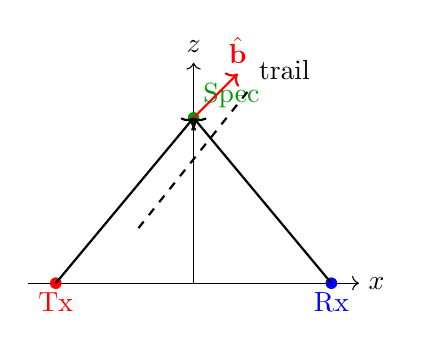
\begin{tikzpicture}[scale=0.7]
    \draw[->] (-3,0) -- (3,0) node[right] {$x$};
    \draw[->] (0,0) -- (0,4) node[above] {$z$};
    \fill[red] (-2.5,0) circle (3pt) node[below] {Tx};
    \fill[blue] (2.5,0) circle (3pt) node[below] {Rx};
    \fill[green!60!black] (0,3) circle (3pt) node[above right] {Spec};
    \draw[thick,dashed] (-1,1) -- (1,3.5) node[above right] {trail};
    \draw[->,thick] (-2.5,0) -- (0,3);
    \draw[->,thick] (2.5,0) -- (0,3);
    \draw[->,thick,red] (0,3) -- (0.8,3.8) node[above] {$\hat{\mathbf{b}}$};
\end{tikzpicture}
\end{column}
\end{columns}
\end{frame}

%---------------------------------------------------
\begin{frame}{Specular Point \& Bistatic Angle}
For each trail point $\mathbf{p}_i$:
\begin{align*}
    \hat{\mathbf{u}}_{\mathrm{Tx}} &= \frac{\mathbf{p}_i - \mathbf{r}_{\mathrm{Tx}}}{|\mathbf{p}_i - \mathbf{r}_{\mathrm{Tx}}|}, &
    \hat{\mathbf{u}}_{\mathrm{Rx}} &= \frac{\mathbf{p}_i - \mathbf{r}_{\mathrm{Rx}}}{|\mathbf{p}_i - \mathbf{r}_{\mathrm{Rx}}|} \\\[0.5em]
    \cos\beta_i &= \hat{\mathbf{u}}_{\mathrm{Tx}} \cdot \hat{\mathbf{u}}_{\mathrm{Rx}}, &
    \hat{\mathbf{b}}_i &= \frac{\hat{\mathbf{u}}_{\mathrm{Tx}} + \hat{\mathbf{u}}_{\mathrm{Rx}}}{|\hat{\mathbf{u}}_{\mathrm{Tx}} + \hat{\mathbf{u}}_{\mathrm{Rx}}|}
\end{align*}

\begin{block}{Key insight}
The specular point minimizes total path length $r_{\mathrm{Tx}} + r_{\mathrm{Rx}}$. \\
The bistatic bisector $\hat{\mathbf{b}}$ sets the Doppler sensitivity direction.
\end{block}
\end{frame}

%===================================================
\section{Physical Model}
%---------------------------------------------------
\begin{frame}{Temporal Envelope: Formation \& Diffusion}
The global amplitude envelope combines rapid formation and gradual diffusion:
\[
E(t) = \underbrace{\bigl[1 - e^{-(t-t_0)/\tau_{\mathrm{rise}}}\bigr]}_{\text{formation}} \cdot
       \underbrace{e^{-(t-t_0-t_{\mathrm{diff}})/\tau_{\mathrm{decay}}}}_{\text{diffusion}} \cdot H(t-t_0)
\]

\begin{center}
\begin{tabular}{lll}
\toprule
Parameter & Value & Physical meaning \\
\midrule
$t_0$ & 2.0 s & Meteor entry time \\
$\tau_{\mathrm{rise}}$ & 5 ms & Trail ionization rise \\
$t_{\mathrm{diff}}$ & 3.0 s & Diffusion onset \\
$\tau_{\mathrm{decay}}$ & 1.0 s & Diffusion time constant \\
\bottomrule
\end{tabular}
\end{center}
\end{frame}

%---------------------------------------------------
\begin{frame}{Wind-Shear Field}
Horizontal wind along the trail is expanded in harmonics:
\[
v(z) = v_{\mathrm{wind}} \Bigl[ r_1 \sin(\pi z) + r_2 \sin(2\pi z) + r_3 \sin(3\pi z) \Bigr]
\]

\begin{columns}
\begin{column}{0.5\textwidth}
\textbf{Parameters:}
\begin{itemize}
    \item $v_{\mathrm{wind}}$ --- overall wind speed (20--150 m/s)
    \item $r_1, r_2, r_3$ --- relative harmonic amplitudes
\end{itemize}
\vspace{0.3em}
The gradient $\mathrm{d}v/\mathrm{d}z$ drives shear deformation over time.
\end{column}
\begin{column}{0.45\textwidth}
\begin{block}{Why harmonics?}
Real atmospheric wind profiles contain multiple scales. \\
Users can dial in $r_2, r_3$ to match observed complex Doppler curves.
\end{block}
\end{column}
\end{columns}
\end{frame}

%---------------------------------------------------
\begin{frame}{Velocity Evolution: Ping $\to$ Shear}
At time $\tau$ after entry, the horizontal velocity interpolates between:
\begin{itemize}
    \item \textbf{Entry ``ping'':} $v_{\mathrm{entry}} = 8\sin(2\pi z) + 15\tan(\mathrm{skew})$
    \item \textbf{Wind shear:} $v(z)$ from the harmonic field
\end{itemize}

\[
v_{\mathrm{hor}}(\tau) = \underbrace{e^{-\tau/0.12}}_{\text{ping decay}} v_{\mathrm{entry}} +
                         \underbrace{\bigl(1 - e^{-\tau/0.40}\bigr)}_{\text{shear growth}} v(z)
\]

\begin{alertblock}{Physical picture}
The head echo (underdense) dies out in $\sim$0.1 s, while the overdense trail is progressively deformed by winds over $\sim$0.4 s.
\end{alertblock}
\end{frame}

%---------------------------------------------------
\begin{frame}{Doppler Shift \& Specular Weighting}
\textbf{Doppler shift} at each trail point:
\[
f_{\mathrm{D},i} = \frac{\mathbf{v}_i \cdot \hat{\mathbf{b}}_i}{\lambda}
\qquad
\mathbf{v}_i = v_{\mathrm{hor},i}\bigl(\cos\epsilon\,\hat{\mathbf{x}} + \sin\epsilon\,\hat{\mathbf{z}}\bigr)
\]

\textbf{Specular weight} (Fresnel-zone-like):
\[
w_i = \exp\!\left[ -\frac{(\mathrm{d}x/\mathrm{d}z)^2}{A(\tau)} \right]
\]
where the aperture broadens with time:
\[
A(\tau) = 0.005 + 0.015\,(1-e^{-\tau/0.40}) + 0.010\,(\tau - 3)\,H(\tau-3)
\]

\begin{block}{Interpretation}
As the trail deforms, the effective specular reflection region widens, reducing coherence and narrowing the Doppler bandwidth.
\end{block}
\end{frame}

%===================================================
\section{Implementation}
%---------------------------------------------------
\begin{frame}{Signal Synthesis Pipeline}
\begin{enumerate}
    \item \textbf{Geometry setup} --- sample 4000 points along $z \in [-1.2, +1.2]$ km
    \item \textbf{Time loop} (15 s at 22.05 kHz):
    \begin{itemize}
        \item Update wind-shear deformation: $\mathrm{d}x/\mathrm{d}z(t)$
        \item Compute Doppler shifts $f_{\mathrm{D},i}(t)$
        \item Accumulate phases: $\phi_i \mathrel{+}= 2\pi(f_c + f_{\mathrm{D},i})\,\Delta t$
        \item Sum weighted sinusoids: $s(t) = E(t) \sum_i w_i \sin\phi_i$
    \end{itemize}
    \item \textbf{Noise injection} (optional Gaussian, configurable SNR)
    \item \textbf{Normalization} and export to WAV / PNG
\end{enumerate}
\vspace{0.3em}
\texttt{Runtime: $\sim$0.5 s per simulation on a modern laptop.}
\end{frame}

%---------------------------------------------------
\begin{frame}{Interactive GUI}
\begin{columns}
\begin{column}{0.5\textwidth}
\textbf{10 sliders:}
\begin{itemize}
    \item Geometry: $d$, $h_{\mathrm{spec}}$, $\alpha$, $\epsilon$
    \item RF: carrier frequency $f_0$ (30--300 MHz)
    \item Trail: skew angle
    \item Wind: speed + 3 harmonic ratios
\end{itemize}
\vspace{0.3em}
\textbf{Controls:}
\begin{itemize}
    \item Noise on/off toggle
    \item Run / Play / Save WAV / Save PNG
\end{itemize}
\end{column}
\begin{column}{0.45\textwidth}
\begin{block}{Two-panel display}
\begin{itemize}
    \item \textit{Left:} 2-D trail geometry at $t = 0, 1.5, 3.0, 4.5, 6.0$ s
    \item \textit{Right:} Spectrogram ($\pm$120 Hz around 1 kHz audio carrier)
\end{itemize}
\end{block}
\end{column}
\end{columns}
\end{frame}

%===================================================
\section{Results}
%---------------------------------------------------
\begin{frame}{Default Parameter Echo}
\begin{columns}
\begin{column}{0.48\textwidth}
\textbf{Settings:}
\begin{itemize}
    \item $d = 50$ km, $h_{\mathrm{spec}} = 90$ km
    \item $f_0 = 50$ MHz, skew $= 12°$
    \item $v_{\mathrm{wind}} = 80$ m/s
    \item $r_1 = 1.00$, $r_2 = 0.00$, $r_3 = 0.10$
\end{itemize}
\vspace{0.3em}
\textbf{Observed morphology:}
\begin{enumerate}
    \item Sharp initial ping at $t \approx 2$ s
    \item Smooth Doppler drift over 2--4 s
    \item Gradual decay and narrowing
\end{enumerate}
\end{column}
\begin{column}{0.48\textwidth}
\fbox{\parbox{\textwidth}{\centering\vspace{2cm} Spectrogram placeholder \vspace{2cm}}}
\end{column}
\end{columns}
\end{frame}

%---------------------------------------------------
\begin{frame}{Parameter Space Exploration}
\begin{columns}
\begin{column}{0.48\textwidth}
\textbf{High 2nd harmonic ($r_2 = 0.8$):}
\begin{itemize}
    \item S-shaped Doppler curve
    \item Two inflection points in drift rate
    \item Mimics observed ``hook'' echoes
\end{itemize}
\vspace{0.5em}
\textbf{High wind speed ($v = 150$ m/s):}
\begin{itemize}
    \item Large total Doppler excursion
    \item Rapid trail deformation
    \item Short echo duration
\end{itemize}
\end{column}
\begin{column}{0.48\textwidth}
\textbf{Large baseline ($d = 150$ km):}
\begin{itemize}
    \item Larger bistatic angle $\beta$
    \item Reduced forward-scatter gain
    \item Weaker but longer-lasting echo
\end{itemize}
\vspace{0.5em}
\textbf{Low elevation ($\epsilon = 10°$):}
\begin{itemize}
    \item Strong vertical velocity projection
    \item Asymmetric Doppler signature
\end{itemize}
\end{column}
\end{columns}
\end{frame}

%===================================================
\section{Conclusion}
%---------------------------------------------------
\begin{frame}{Summary \& Future Work}
\textbf{What \texttt{echoSim} provides:}
\begin{itemize}
    \item First-principles forward-scatter geometry
    \item Multi-harmonic wind-shear-driven trail deformation
    \item Real-time audio + spectrogram synthesis
    \item Open, hackable Python codebase
\end{itemize}

\vspace{0.5em}
\textbf{Planned extensions:}
\begin{itemize}
    \item Fresnel-zone diffraction for underdense regime
    \item HWM14/ empirical wind model coupling
    \item Multi-station network geometry
    \item Batch Monte-Carlo parameter sweeps
\end{itemize}
\end{frame}

%---------------------------------------------------
\begin{frame}
\begin{center}
\Huge Thank You!
\vspace{1cm}

\Large Questions?
\vspace{1.5cm}

\normalsize
\texttt{echoSim} source code available at: \\
\texttt{https://github.com/\dots/echoSim} (placeholder)
\vspace{0.5em}

Contact: \texttt{author@institution.edu}
\end{center}
\end{frame}

\end{document}
